\section{Experimental Results}
\label{sec:experiments}

We evaluate the performance of the \term{fast subsequence matching} algorithm and the \term{KNN} algorithm, separately.
Then we evaluate the performance of the integrated algorithm which harmonizes the two algorithms. 

\subsection{Experimental Setup}
\label{sec:experimental_setup}

The \term{Samsung Galaxy S} device running \term{Android 2.3 Gingerbread} and the \term{Netflix} application are used for our experiments. 
10 movies are selected from the \term{Popular on Netflix} section of the Netflix website and the selected movies are shown in the Table \ref{tab:movies}.
CPU usage sequences of the movies are captured by recording CPU usage statistics in 1-second and 5-second intervals using the native UNIX/Android command, \term{top}, while playing the first 30 minutes of each movie. 
The measurement is repeated 5 times for each movie.
The preliminary measurement results of two selected movies are previously shown in Figure \ref{fig:preliminaries}.

\begin{table}[!t]
\begin{center}
\begin{tabular}{|c | m{5cm} ||c| m{5cm}|}
\hline
ID & Movie Title & ID & Movie Title \\ 
\hline
1 & Transformers: Dark of the Moon 		& 6 & Super 8\\
2 & Thor					& 7 & Mean Girls 2 \\
3 & Hachi: A Dog's Tale 			& 8 & Captain America \\
4 & The True Story of Puss 'n Boots 		& 9 &  Snatch \\
5 & Wallace \& Gromit: Loaf and Death 	& 10 & No Strings Attached \\
\hline
\end{tabular}
\end{center}
\caption{10 Movies selected from \term{Popular on Netflix}}
\label{tab:movies}
\end{table}

For each movie, one out of five raw sequences is selected as \term{query sequence} and the rest are considered \term{training sequences}.
Then query sequence and training sequences are preprocessed both in the fast subsequence matching algorithm and the KNN algorithm. 
In the fast subsequence matching algorithm, a query sequence and training sequences are preprocessed and converted into space-series sequences separately through DFFT.
Then query sequence is divided into several query subsequences and the fast subsequence matching algorithm predicts the movie title of each query subsequence. 
In KNN algorithm, a query sequence is divided into several query subsequences and then training sequences are also divided into subsequences of the same length as query subsequences. 
Then KNN algorithm predicts the movie title of each query subsequence. 
These procedures are depicted in Figure \ref{fig:train_test_set}.

\begin{figure}[!t]
\centering
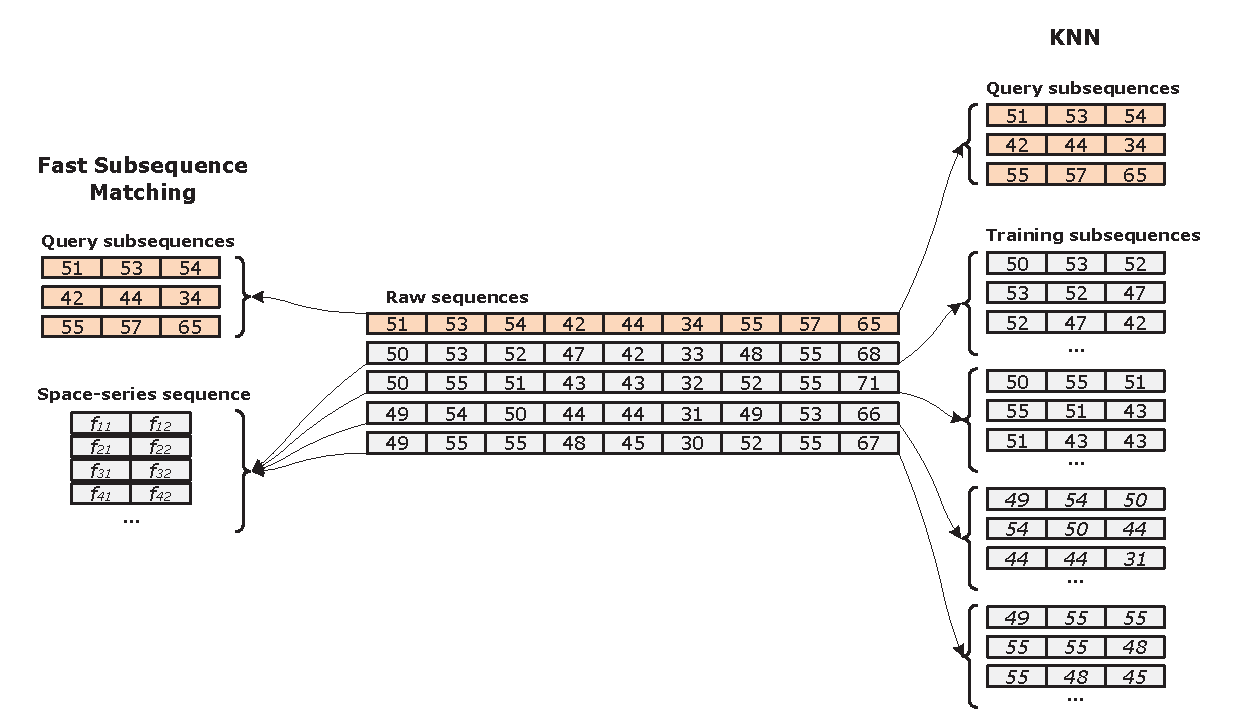
\includegraphics[scale=0.60]{Figures/TrainTestSet}
\caption{Preprocessing of raw sequences in Fast Subsequence Matching algorithm and KNN algorithm}
\label{fig:train_test_set}
\end{figure}

\subsection{Fast Subsequence Matching Algorithm Results}
Query subsequences are chosen from a 30-min length sequence with varying starting index and length. At every 60-second interval, subsequences are selectd with length, $l =$ [180, 240, 300, 600, 900, and 1200] (3, 4, 5, 10, 15, 20 minutes). For each selected query subsequence, various lengths of the Discrete Fourier Transform window are applied to find the best performance configuration. The DFT window with length, $w=$ [50, 100, 150, 200, 300], are applied to extract the two lowest Fourier coefficient ($f=2$). The DFT window length affects the performance of the matching algorithm. If the length of the DFT window is too short, then DFT procedure will result in high noise sensitivity. Otherwise, the DFT procedure results in over-smoothing of the data.

The performance of the matching algorithm is measured by the rate of the number of correct predictions to the number of total queries.
\begin{equation}
R_{succ} = \frac{\#\: of \:correct\: predictions}{\# \:of\: total \:predictions}
\end{equation}

\subsubsection{Success Rate:} The Table \ref{tab:succ_table} shows the success rate of the matching algorithm with varying query sequence length and varying DFT window size. It's obvious that the success rate increases as the length of query sequences goes large. As shown in the Table \ref{tab:succ_table}, the success rate increases as the sequence length increases when the size of DFT window is fixed. With the collected database sequences, our matching scheme gives the best prediction performance when the DFT window length is 200. However, it is impossible to apply DFT procedure with the window lenght 200 to query sequences that are shorter than DFT window length. Those entries in the Table are marked as non-applicable. 


\begin{table}[h!]
\begin{center}
\begin{tabular}{|c|| >{\centering} p{1cm}| >{\centering} p{1cm}| >{\centering}p{1cm}| >{\centering}p{1cm}| >{\centering}p{1cm} |}
\hline
Seq Len ($l$) \textbackslash FFT Len ($w$)& 50 & 100 & 150 & 200 & 300
\tabularnewline
\hline
180 & 0.46 & 0.54 & 0.62 & N/A & N/A
\tabularnewline
240 & 0.475 & 0.585 & 0.64 & 0.655 & N/A
\tabularnewline
300 & 0.52 & 0.595 & 0.665 & 0.65 & 0.69
\tabularnewline
600 & 0.705 & 0.69 & 0.75 & 0.747 & 0.74
\tabularnewline
900 & 0.726 & 0.7428 & 0.8 & 0.791 & 0.72
\tabularnewline
1200 & 0.78 & 0.755 & 0.7875 & 0.814 & 0.74
\tabularnewline
\hline
\end{tabular}
\end{center}
\caption{Success Rate of Prediction}
\label{tab:succ_table}
\end{table}

\subsubsection{Confidence of Prediction:} The fast subsequence matching algorithm provides the result very fast in short execution time with considerable accuracy over 70\% when the DFT window length is 200. This efficiency comes from the fact that the algorithm exploits only the two lowest frequencies ($f=2$) of (sub-)sequences extracted by DFT to predict the title of the movie. However, the efficiency in the execution time compromises the confidence of our prediction. Thus, we define the confidence of the succerate as follows.
\begin{equation}
C = \frac{\#\: of \:correct\: query\: responses}{\# \:of\: total \:query\: responses}
\end{equation}

$C$ is defined as the rate of correct query responses to total query responses. At each query, the algorithm returns multiple number of responses that may be correct or wrong prediction because the data structure, R* Tree, searches each MBR within some threshold distance from the query and returns multiple nodes that correspond to response. Thus, $C$ can be regarded as true positive rate of query responses. The Table \ref{tab:tp_table} shows $C$ with the DFT window length, $w =$ [150, 200, 300].

\begin{table}[h!]
\begin{center}
\begin{tabular}{|c|| >{\centering} p{1cm}| >{\centering} p{1cm}| >{\centering}p{1cm}|}
\hline
FFT Len ($w$)& 150 & 200 & 300
\tabularnewline
\hline
Average & 0.487 & 0.539 & 0.610 
\tabularnewline
\hline
\end{tabular}
\end{center}
\caption{Confidence of Prediction}
\label{tab:tp_table}
\end{table}

As shown in the Table \ref{tab:tp_table}, the $C$ is around 50 percent for the DFT length 150 and 200, and 61 percent on average for the DFT length 300. The results show that the correct prediction occupies more than 50 percent of total response while the other 9 movie sequences occupy rest of the total responses. In most cases, the number of the correct prediction usually dominates the second best prediction of the algorithm. However, there're still cases where the correct prediction and the second best prediction are not differenciated by the number of query responses. For example, if the correct prediction takes 40\% of the total query responses and the second best prediction takes 30\% of the total query responses, then it may be hard to say that our prediction has a high confidence. Thus, the prediction scheme needs to be enhanced to deal with the case when the difference of $C$ is small.
\subsection{KNN Results}

For each movie, one of five CPU usage sequences is selected as query sequence and the rest four sequences are considered training data set, as described in \ref{sec:experimental_setup}, 
The length of subsequence varying from 60 seconds to 360 seconds is set and each test and training data is divided based on the subsequence length as described in \ref{sec:knn}.
When dividing sequence data, we adopt a concept of sliding window which moves by 1 step size.
Each data sequence consists of $360$ measurement points, and therefore $(360 - subsequence\_length + 1)$ subsequences are generated from the data sequence. 

After building up test data set and training data set by generating subsequences, we apply KNN method in order to classify each subsequence of test data based on training data set. 
In this experiment, $k$ value is set to 3 for the simplicity.
The accuracy of classification according to the length of subsequence is shown in Figure \ref{fig:experiment_knn}.
The accuracy is low as 46$\%$ when subsequence length is set to 60-second.
However, the accuracy increases up to 88$\%$ when subsequence is set to 180-second.
The experimental result shows that given 10 movies and CPU usage statistics of 150 seconds, our side channel attack correctly predicts which movie a user is watching at the accuracy of higher than 80$\%$.

\begin{figure}[!h]
\centering
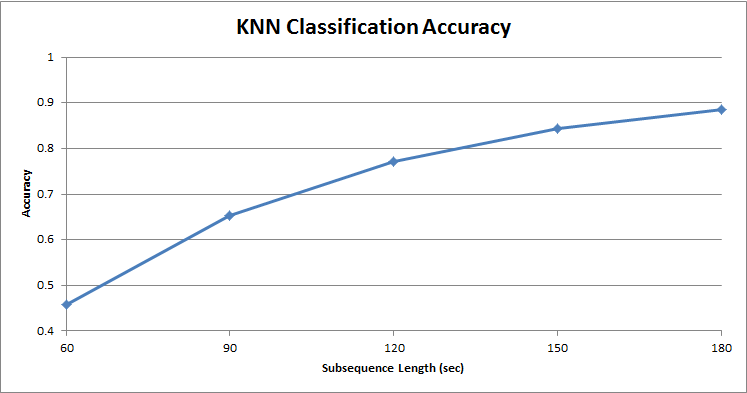
\includegraphics[scale=0.50]{Figures/experiment_knn}
\caption{KNN Classification Accuracy}
\label{fig:experiment_knn}
\vspace{-5mm}
\end{figure}
\subsection{Unified Algorithm Results}

Unified algorithm here.

\subsubsection{Execution Time:} The execution time of the fast subsequence matching algorithm is measured from pre-processing a query subsequence (i.e. smoothing, DFT, packing MBR) to assessing final query responses. The execution time is measured when the DFT window length is 150. The reason for the selection is that 1) the window length provides one of the best prediction results and 2) various sequence lengths can be tested. 
The execution time of the KNN algorithm is measured after $n$ candidates filtered by the FSM are delivered to the KNN algorithm as the input parameters. In the experiment, the execution times of $n = [10, 4, n_{90}$ were measured where $n_{90}$ refers to the number of candidates that occupy 90\% of the total response from the FSM.


\begin{table}[h!]
\begin{center}
\begin{tabular}{|c|| c| c| c| c| }
\hline
Seq Len & Fast Subsequence Matching & KNN +FSM (n=10) & KNN + FSM (n=4) & KNN + FSM (90\%)
\tabularnewline
\hline
180 & 1.70 & 33.24 & 16.75 & 16.92
\tabularnewline
240 & 1.74 & 32.32 & 16.31 & 17.16 
\tabularnewline
300 & 1.88 & 33.04 & 16.88 & 18.06 
\tabularnewline
600 & 2.13 & 28.85 & 15.36 & 17.77
\tabularnewline
900 & 2.48 & 24.43 & 13.86 & 15.95
\tabularnewline
1200 & 2.80 & 19.13 & 11.67 & 13.27
\tabularnewline
\hline
\end{tabular}
\end{center}
\caption{Execution Time Measurement}
\label{tab:exec_table}
\end{table}



